% =====================================================================================
\section{Method}
\label{sec:method}
% =====================================================================================

\begin{figure}[t]
\centering
\begin{tikzpicture}[font=\scriptsize, node distance=3mm,
  sem/.style={draw, rounded corners=2pt, fill=gray!10, align=center, inner sep=3pt},
  orc/.style={draw, rounded corners=2pt, fill=blue!6, align=center, text width=24mm, inner sep=3pt},
  sys/.style={draw, rounded corners=2pt, fill=orange!10, align=center, text width=18mm, inner sep=3pt},
  arr/.style={-{Stealth[length=1.5mm]}, semithick}]
  \node[sem, text width=74mm] (S) {\textbf{Reference semantics}: rule chain and requirements written once\\
    as guards over an environment and a logic interface};
  \node[sem, below left=4mm and -24mm of S, text width=19mm] (py) {Python\\booleans};
  \node[sem, right=3mm of py, text width=19mm] (z3) {z3 terms\\(unbounded)};
  \node[sem, right=3mm of z3, text width=19mm] (ce) {Cedar policies\\(validated, \S\ref{sec:rq5})};
  \foreach \n in {py,z3,ce} \draw[arr] (S.south -| \n.north) -- (\n.north);
  \node[orc, below=6mm of py] (o1) {\textbf{L1} differential check\\+ criterion G\\+ coverage (SMT)};
  \node[orc, right=3mm of o1] (o2) {\textbf{L2} cold-cache check,\\staleness, races\\(Thm.~\ref{thm:stale})};
  \node[orc, right=3mm of o2] (o3) {\textbf{L3} path inventory,\\probes, ledger counts};
  \draw[arr] (py) -- (o1); \draw[arr] (z3.south) -- (o1.north east);
  \draw[arr] (py.south east) -- (o2.north west);
  \node[sys, below=6mm of o1] (pdp) {PDP code};
  \node[sys, below=6mm of o2] (st) {DB + grant cache};
  \node[sys, below=6mm of o3] (pep) {PEPs, other paths,\\audit ledger};
  \draw[arr] (o1) -- (pdp); \draw[arr] (o2) -- (st); \draw[arr] (o3) -- (pep);
\end{tikzpicture}
\caption{The method. One reference semantics, three interpretations, and one oracle per level, each running
the corresponding part of the deployment for real.}
\label{fig:method}
\end{figure}

\paragraph{One semantics, three readings.} We write each chain once, as a list of (rule, effect, guard)
triples whose guards are functions of an abstract environment and a logic interface. Evaluated with Python
booleans, the code is a test oracle. Evaluated with z3 \cite{demoura2008z3} terms over uninterpreted sorts, it
yields proofs for any number of departments, divisions and actions. Evaluated as Cedar expressions, it compiles
to Cedar policies (\S\ref{sec:rq5}). Because the three share code, the proofs are about the very semantics
the tests compare against the implementation.

\paragraph{L1: making a bounded check complete.} The L1 oracle runs the \emph{unmodified} PDP, including the
code that builds its context, over a bounded world space $W$, and compares the decision and the deciding rule
with $\mathcal{M}$. Only the data sources are replaced: the grant cache returns the world's grant sets. The
obvious objection is that $W$ is small. The answer is that the PDP cannot tell apart worlds that look the same
through a fixed set of observations. Let the \emph{observation vector} of a world be
\[
\obs(w)=\bigl(\role(u),\kappa_C(\mathsf{clr}(u)),\kappa_S(\mathsf{sens}(o)),\,b_1,\dots,b_9\bigr)
\]
where $b_1,\dots,b_9$ are the Boolean atoms $\sameDept$, $\mathsf{div}(u)=\bot$, $\sameDiv^\circ$,
$\rho\ge\theta$, $a=\mathit{read}$, $a\in\Gasg_t$, $a\in\Gdel_t$, $\Gasg_t\neq\emptyset$ and $\Gdel_t\neq\emptyset$.
We write $\mathcal{M}$ and $R$ over these atoms and, for the owner exception, two more,
$[\mathsf{own}(o)=u]$ and $[a=\mathit{download}]$; the v1 PDP reads neither, and the v2 PDP reads both
(\S\ref{sec:rq5}).

\emph{Criterion G.} G fixes the language the decision code may use. (a) Every value of an open sort
(departments, divisions, identifiers, actions, grant sets) may be used only through an observation: equality,
inequality or \texttt{is None} against a non-constant term of the same sort; comparison of the action with a
constant that obs represents (\emph{read}, and for v2 also \emph{download}); membership of the action in a grant set; non-emptiness of a
grant set. (b) A closed attribute may be read only if obs represents it (role, clearance, sensitivity, the
administrator flag). (c) The request context may only be passed to the risk helper, whose result is compared only
with the threshold, or flow into sinks. (d) Anything else may flow only into sinks (strings, the trace, logs, the
audit snapshot), including branches that write only sinks; no other branch condition reads a sink. (e) A helper
that receives a whole entity must not read it at an open-sort attribute.

\begin{lemma}[Data independence]\label{lem:di}
Let the decision procedure be loop-free and satisfy G (a)--(e), checked over its decision functions and every
helper that receives an entity, and assume the language's semantics of equality and membership. Then there is a
function $g$ with $\mathcal{I}(w)=g(\obs(w))$ for all worlds $w$, whatever the size of the domains.
\end{lemma}
\begin{proof}
Take two worlds $w_1,w_2$ with $\obs(w_1)=\obs(w_2)$ and run $\mathcal{I}$ on both in lockstep. We show by
induction on the number of executed statements that both runs execute the same statements, and that at each
point every variable of a closed sort holds the same value in both runs. Initially this holds trivially. A
statement can change control flow only through a branch condition. By G, each atomic sub-expression of a
condition is either a closed value, which is equal in both runs by the induction hypothesis, or an observation.
Every observation in the checked code compares attributes of the request's own subject, object and action, or
the grant sets that the key lookups return for that subject and object. Its value is therefore one of the
atoms of $\obs$, and equal in both runs. Values that reach sinks are never read by a condition. A helper that
receives an entity reads only closed attributes, so its result, which the PDP compares only with the risk
threshold, is again an atom. Hence every condition evaluates identically, the runs take the same path, and
they return the same decision and rule. Since the code is loop-free, the induction is over a finite path. This
is the classical data-independence argument \cite{wolper1986,lazic2003semantic}, specialized to one decision.
\end{proof}

\begin{theorem}[Completeness of bounded checking]\label{thm:complete}
Let $V_{\mathrm{sat}}$ be the set of observation vectors satisfiable over unbounded domains. If
$V_{\mathrm{sat}}\subseteq\obs(W)$ and $\mathcal{I}(w)=\mathcal{M}(w)$ for all $w\in W$, then
$\mathcal{I}=\mathcal{M}$ on all worlds, and a requirement is violated by some world if and only if it is violated
in $W$.
\end{theorem}
\begin{proof}
Given any $w$, pick $w'\in W$ with $\obs(w')=\obs(w)$. Then $\mathcal{I}(w)=g(\obs(w))=\mathcal{I}(w')=
\mathcal{M}(w')=\mathcal{M}(w)$, and every requirement is a function of $\obs$ and the decision.
\end{proof}

Algorithm~\ref{alg:l1} puts the pieces together. Both premises of Theorem~\ref{thm:complete} are checked by
tools, not argued. An AST checker verifies G and exports a certificate: every occurrence of an open-sort value
with its observation class, the accepted language, and the action constants it admits. To make sure the checker
is not vacuous, we planted ten violations: an ordering on departments, a string operation on the action, the
cardinality of a grant set, a hash of a division, a sink read inside a condition, a risk helper that reads the
department, a comparison with a department constant, a comparison with an action constant that obs does not
represent, a closed attribute outside obs in a condition, and a context value deciding outside the risk helper.
Our first checker accepted the last three; the
revised checker flags all ten, in the PDP of v1 and in that of v2, and still accepts both unmodified PDPs. A z3 enumeration lists the satisfiable observation vectors and compares them with those that
$W$ realizes. Counts of violating worlds stay specific to $W$. What transfers is whether a requirement holds at
all.

\begin{algorithm}[t]
\caption{Complete bounded L1 check}
\label{alg:l1}
\KwIn{PDP code $\mathcal{I}$; chain $\mathcal{M}$; requirements $R$; world space $W$}
\lIf{criterion G fails on $\mathcal{I}$ \textnormal{(AST check)}}{\Return the violating occurrences}
$V_{\mathrm{sat}}\gets\{v\mid v \text{ satisfiable in z3 over uninterpreted sorts}\}$\;
$V_W\gets\{\obs(w)\mid w\in W\}$\;
\lIf{$V_{\mathrm{sat}}\not\subseteq V_W$}{\Return the missing vectors, and extend $W$}
\ForEach{$w\in W$}{
  load subject and object of $w$; stub grant cache with $(\Gasg,\Gdel)(w)$\;
  $(d,r)\gets\mathcal{I}.\decide(w)$ \tcp*{real PDP code}
  \lIf{$(d,r)\neq\mathcal{M}(w)$}{report a transcription mismatch}
  \ForEach{$\phi\in R$}{\lIf{$\neg\phi(w,d)$}{record a violation and a minimal witness}}
}
prove or refute each $\phi\in R$ for $\mathcal{M}$ with z3 over uninterpreted sorts\;
\end{algorithm}

\paragraph{L2: state.} The \emph{cold-cache} oracle inserts grants in every lifecycle state into the real
database and compares the PDP's queries, with an empty cache, against $\Gasg_t$ and $\Gdel_t$. With the cache
in place, the question becomes how stale a decision can be. For the plain TTL cache that \sysname v1 and most
applications use, the answer is exact.

\begin{theorem}[Bounded staleness, per component]\label{thm:stale}
Suppose the cache stores, per pair $(u,o)$ and grant kind $g$, the action set read from committed state at $t_r$,
writes it at $t_w\le t_r+\epsilon$ with lifetime $\tau_g$, and checks validity bounds only on a miss, while
attributes are read from committed state at decision time. Then every decision at $t$ reads, for each $g$,
$G^g_{t_g}(u,o)$ for some $t_g\in(t-\tau_g-\epsilon,t]$: the deployment is L2$^c_{\tau+\epsilon}$ with
$\tau=\max_g\tau_g$. Let a grant of kind $g$ stop holding at $t_{\mathrm{end}}$ without invalidating the cache (by
expiry, or by a revocation that does not invalidate), and let the live entry for $(u,o,g)$ have age
$\delta\in[0,\tau_g)$ at $t_{\mathrm{end}}$. If that entry is neither refilled nor invalidated before it expires,
it keeps returning the ended grant for exactly $\tau_g-\delta$ after $t_{\mathrm{end}}$, and a request that only
this grant allows is allowed for that long. Invalidating \emph{before} the commit does not improve the worst case,
and the bound is tight.
\end{theorem}
\begin{proof}
A live entry was read at $t_r\ge t_w-\epsilon>t-\tau_g-\epsilon$; on a miss $t_g=t$. An entry holding an ended grant
was read before $t_{\mathrm{end}}$ and, untouched, lives until $t_w+\tau_g=t_{\mathrm{end}}+\tau_g-\delta$; whether
the request is allowed then depends on that grant only if no other grant or rule allows it. A read that falls
between an invalidation and the commit stores the old state again, for a full $\tau_g$. For tightness, take a
read just before $t_{\mathrm{end}}$.
\end{proof}

A componentwise bound is not a bound on the state a decision uses. Two cached grant sets may come from
different committed states, and a chain may combine them.

\begin{proposition}[Mixed views]\label{prop:mixed}
With per-component caches as in Theorem~\ref{thm:stale}, \chain is L2$^c_{\tau+\epsilon}$ but not L2$^+_\Delta$
for any $\Delta$: some API-reachable run contains an allow that $\mathcal{M}$ gives in no committed state.
\end{proposition}
\begin{proof}
Let $u$ be an employee of another department than $o$. At $t_0$ the object's director assigns $u$
$\{\mathit{write}\}$ until $t_0+10$\,s, and a write decision caches $\Gasg=\{\mathit{write}\}$ for $\tau_{\mathrm{asg}}=120$\,s
and $\Gdel=\emptyset$ for $\tau_{\mathrm{del}}=60$\,s ($P_1$ denies). The assignment expires; after the
delegation entry has expired, a read delegation is approved, which invalidates nothing. A write decision now reads
$\Gdel=\{\mathit{read}\}$ from the database and $\Gasg=\{\mathit{write}\}$ from the cache: $P_1$ passes and $P_4$
allows. The committed states of the run are $(\{\mathit{write}\},\emptyset)$, $(\emptyset,\emptyset)$ and
$(\emptyset,\{\mathit{read}\})$, in which $\mathcal{M}$ denies by $P_1$, $P_1$ and $P_5$.
\end{proof}

The hazard needs a chain that combines grant kinds; $\mathcal{F}$ does not.

\begin{proposition}[Single witness]\label{prop:witness}
Suppose that every allow rule's guard reads at most one grant set, and that every deny rule before it either reads
no grant set or is false whenever that guard is true. Then for each allow decision computed on a view, the
committed state $\sigma_{t_g}$ of the grant set $g$ that the deciding rule reads also yields an allow, provided the
attributes of $u$ and $o$ did not change in $(t_g,t]$. $\mathcal{F}$ satisfies the premise; \chain does not, since
$P_1$ reads $\Gdel$ and the later $P_4$ reads $\Gasg$.
\end{proposition}
\begin{proof}
Let rule $r_i$ decide the view with allow. In $\sigma_{t_g}$ the attributes and the grant set $r_i$ reads are as in
the view, so $\gamma_i$ holds; every earlier deny rule reads no grant set (and so evaluates as in the view, to
false) or is false because $\gamma_i$ is true. So the first applicable rule in $\sigma_{t_g}$ is an allow rule.
In $\mathcal{F}$, $\Px$ and $\Pc$ read no grant set, $P_1$ is false when $P_2$, $P_3$, $\Po$ or $P_4$ applies
($\sameDept$) and when $P_6$ applies ($\Gdel\neq\emptyset$), and ADMIN, $P_2$, $P_3$ and $\Po$ read no grant set.
\end{proof}


The \emph{staleness} experiments test this prediction. They warm the cache $\delta$ seconds before a grant ends,
end it by revocation or by expiry, and poll the decision API at 4\,Hz until it denies. For
races, we revoke while decisions are in flight, once in-process with a single decision injected between cache
invalidation and commit, and once under a two-worker server with real parallelism.

\paragraph{L3: enforcement.} We list every route that returns protected content, changes grants or opens a
session, note which decision procedure it uses, and probe each one on the running system with fixtures chosen
to make the procedures disagree. For accountability, we count durable ledger rows after allowed and denied
requests. Algorithm~\ref{alg:l3} summarises the procedure. The inventory is generated from the web framework's
routing table, and a static pass over each handler records which decision procedures it can reach; paths outside
the routing table (another process, such as the collaboration server, or scheduled jobs) are added by hand. Two
sweeps complement the probes: every in-scope route is sent, with the identifiers of real objects, by subjects who
must be refused, and any success that reveals content or changes the database is flagged. Each check is either a \emph{safety} check (the PDP denies, so no effect may happen) or a
\emph{liveness} check (the PDP allows, so the effect must happen); the second kind keeps a fix from passing by
simply refusing everything.

\begin{algorithm}[t]
\caption{L3 conformance check}
\label{alg:l3}
\KwIn{running system; PDP $\decide$; administrative policy $\Pi_{\mathrm{adm}}$; requirements $R$}
\ForEach{route $r$ of the generated inventory that returns protected content, changes state, or opens a session}{
  record $D_r$, $\alpha_r$, $\mathit{Ob}_r$, and where $r$ writes its record\;
  \lIf{$D_r\neq\decide$ or $\alpha_r$ depends on $a_c$}{choose fixtures $w$ with $D_r(w)\neq\decide(w)$}
  add fixtures for each guard of $D_r$ and for each $\phi\in R$ that $r$ can affect\;
}
\ForEach{route $r$ and fixture $w$}{
  load $w$ into the database; send the request as the subject of $w$\;
  \lIf{$\decide(w)=\denyv$}{\textbf{safety}: expect no content and no state change}
  \lElse{\textbf{liveness}: expect the effect, and every obligation enforced}
  after the response, count decision and audit rows for the request (expect one each)\;
}
\ForEach{in-scope route $r$ and subject $u$ whom R forbids every action on the fixture's objects}{
  send $r$ as $u$; \textbf{flag} a success that returns marked content or changes the database\;
}
\end{algorithm}

\paragraph{Adequacy.} We apply first-order mutation (relational, connective, negation, membership, constant,
effect and condition operators) to the decision logic, and separately to the enforcement and cache code. Each
mutant is judged by our repository's tests and by each level's oracle. A mutant is \emph{killed} if at least one
test or oracle fails on it, and \emph{survives} otherwise; the \emph{mutation score} is the share of
non-equivalent mutants killed. Since an oracle built while studying survivors can fit the operators it was
tuned on, we also apply a held-out set of operators (statement deletion, swallowed exceptions, swapped
arguments) to the frozen L3 probe. Table~\ref{tab:real} shows which parts
of the system each oracle actually runs, which largely predicts what it can catch.

\begin{table}[t]
\caption{What each oracle runs for real (\ok), stubs ($\circ$), or does not touch (--).
$^\ast$The integration tests turn off the cache client in every PDP test.}
\label{tab:real}
\small
\begin{tabular}{@{}l@{\;}c@{\;\;}c@{\;\;}c@{\;\;}c@{\;\;}c@{}}
\toprule
Oracle & chain & queries & cache & PEP & ledger \\
\midrule
Repo.\ unit / ``conformance'' tests & \ok & $\circ$/-- & $\circ$/-- & -- & $\circ$ \\
Repo.\ integration tests & \ok & \ok & --$^\ast$ & \ok & \ok \\
L1 differential (E1) / SMT (E6) & \ok/model & -- & $\circ$ & -- & -- \\
L2 cold cache (E1b) & \ok & \ok & \ok & -- & -- \\
L2/L3 running system (E2, E5) & \ok & \ok & \ok & \ok & \ok \\
\bottomrule
\end{tabular}
\end{table}

\paragraph{Setup.} Python 3.12.3, FastAPI 0.115.5, SQLAlchemy 2.0.36, PostgreSQL 16.15, Redis 7.0.15, z3
5.3.3 and cedarpy 4.12.2, on a container with 2 vCPUs and 8\,GB. Fixtures go through the API of \sysname
wherever an endpoint exists, and through the ORM otherwise.

% =====================================================================================
\section{Evaluation}
\label{sec:eval}
% =====================================================================================

This section answers the five questions of \S1 in turn. Each subsection ends with a short answer.

\subsection{RQ1: The Rule Level}
\label{sec:l1}

\paragraph{Is the check complete?} Criterion G holds for the v1 PDP: 82 open-sort occurrences, no violation,
and three places where an entity is passed to a helper, all of them checked. The coverage step then caught us
out. The world space we had used until then missed two kinds of state: custom roles, which administrators can
create, and an object in another department that carries the subject's division identifier, which the API does
not prevent. After adding both (Table~\ref{tab:world}), $W$ realizes all 1{,}440 satisfiable combinations of
role and Boolean atoms, and all 864 that are API-reachable (Figure~\ref{fig:l1}b); clearance and sensitivity
are enumerated in full. By Theorem~\ref{thm:complete}, the results below hold for domains of any size.
Table~\ref{tab:verdict} summarises them.

\begin{table}[t]
\caption{World space $W$ of the L1 check. API-reachable means $\Gdel\subseteq\{\mathit{read}\}$ and every
division manager has a division; the PAP enforces both.}
\label{tab:world}
\small
\begin{tabular}{@{}lrl@{}}
\toprule
Dimension & $|\cdot|$ & Values \\
\midrule
role & 5 & adm, dir, dm, emp, cust \\
subject division & 2 & $v_1$, $\bot$ \\
object dept./div. & 6 & same: $v_1,v_2,\bot$; other: $v_3,\bot,v_1$ \\
clearance $\times$ sensitivity & 12 & $C\times S$ \\
$\Gasg$, $\Gdel$ & 64 & $2^{\{\mathit{read},\mathit{write},\mathit{download}\}}$ each \\
action & 4 & read, write, download, delete \\
risk & 2 & $\rho=0$, $\rho=70$ \\
\midrule
total / API-reachable & & 368{,}640 / 82{,}944 \\
\bottomrule
\end{tabular}
\end{table}

\begin{table}[t]
\caption{Verdicts for the requirements of Table~\ref{tab:req}. Impl.: \chain v1 under API-reachable states.
Doc.: our design specification $\mathcal{S}_{\mathrm{doc}}$. v2: the repaired chain $\mathcal{F}$ (\S\ref{sec:rq5}).
\ok\ proved for unbounded domains (z3); \no\ counterexample, with the number of API-reachable violating worlds.
For v2, LP is proved with the owner exception $\ow$; without it, the owner rule violates LP by design.}
\label{tab:verdict}
\small
\begin{tabular}{@{}l@{\;}p{3.9cm}@{\;}c@{\;}c@{\;}c@{}}
\toprule
 & Requirement & Impl. & Doc. & v2 \\
\midrule
R1 & isolation & \ok & \ok & \ok \\
R2 & classification & \ok & \ok & \ok \\
R3 & need-to-know & \ok & \no & \ok \\
R4 & delegation suffices & \no\,108 & \no & \ok \\
R5 & cross-dept.\ only via delegation & \no\,1{,}296 & \ok & \ok \\
R6 & risk & \no\,9{,}876 & \no & \ok \\
R7 & every allow within some rule's scope & \ok & \no & \ok \\
\midrule
LP & employee least privilege & \no\,864 & \ok & \ok \\
\bottomrule
\end{tabular}
\end{table}

\begin{figure*}[t]
\centering
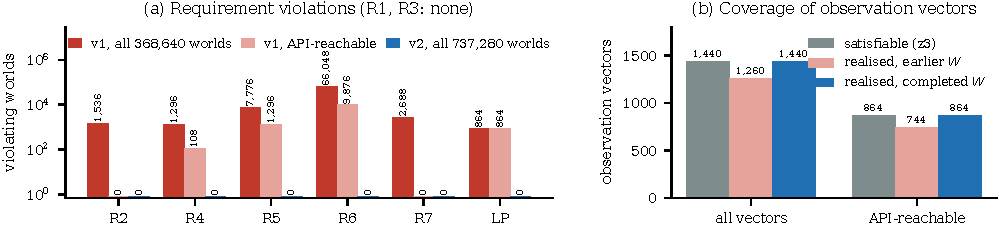
\includegraphics[width=0.9\textwidth]{figs/fig_l1.pdf}
\caption{L1 results. (a) Worlds violating each requirement, for v1 over all worlds, v1 over API-reachable worlds
(the counts of Table~\ref{tab:verdict}), and v2 over all worlds; LP is the employee least-privilege requirement,
with the owner exception of C3. (b) Observation vectors: satisfiable over unbounded
domains (z3), and realised by the world space we used before and after the coverage check.}
\label{fig:l1}
\end{figure*}

\paragraph{Fidelity and drift.} On all 368{,}640 worlds the PDP returned the decision and the deciding rule of
$\mathcal{M}$, without a single indeterminate result (24.5\,s). Our design specification disagrees with it on
18{,}960 worlds. D1 explains all 4{,}032 API-reachable disagreements: the code grants any action in the
assignment, and denies \emph{read} to a subject whose assignment omits it. D2 matters only for division
managers without a division. If the PAP did not forbid those, the D2 exemption would let them past $\Pc$ in
1{,}536 worlds (the R2 bar of Figure~\ref{fig:l1}a), so R2 currently depends on an administrative check.

\begin{theorem}[What v1 gets right]\label{thm:pos}
Under API-reachable states, \chain satisfies R1, R2, R3 and R7 for every number of departments, divisions and
actions.
\end{theorem}
\begin{proof}
Let $\role(u)\neq\mathrm{adm}$. \emph{R1:} its premise is the guard of $P_1$, the first rule that can fire.
\emph{R2:} managers have a division, so $\sameDiv^\circ=\sameDiv$ wherever $\Pc$ applies, and no allow rule
comes before $\Pc$. \emph{R3:} for an employee, $P_4$ needs $a\in\Gasg_t$ and $P_6$ needs $a\in\Gdel_t$.
\emph{R7:} each of the guards of $P_2$, $P_3$, $P_4$ and $P_6$ implies one disjunct. z3 confirms all four with
uninterpreted sorts, including the custom role, in under 10\,ms each.
\end{proof}

\begin{proposition}[The risk rule never changes a decision]\label{prop:inert}
For all $u,o,a$ and all contexts $c,c'$ that differ only in risk signals,
$\pi_d(\decide_{\sigma,t}(u,o,a,c))=\pi_d(\decide_{\sigma,t}(u,o,a,c'))$, where $\pi_d$ projects a result onto
its decision.
\end{proposition}
\begin{proof}
Every allow rule comes before $\Px$, and no guard before $\Px$ mentions $\rho$. So the first applicable rule
among those before $\Px$ is the same in both contexts. If it is an allow rule or an earlier deny rule, both
results agree. Otherwise both evaluations reach $\Px$, and whether $\Px$ or $P_7$ then applies, both deny.
\end{proof}
The \emph{deciding rule} can differ: a custom-role subject without grants is denied by $P_7$ at low risk and by
$\Px$ at high risk. What the proposition rules out is that risk ever turns an allow into a deny.
All 184{,}320 pairs of worlds that differ only in risk get the same decision. Case (c$_2$) of the running
example is one of them. Reading C2 the other way (``risk denies only requests that no allow rule matches'')
does not help: R6 then holds, but only because $P_7$ already implies it, so the rule is dead under either
reading. Our own unit test for $\Px$ passes \emph{because} of this: it checks that a low-risk director is
allowed, which $P_2$ settles first.

\begin{proposition}[A read delegation unlocks writes]\label{prop:unlock}
In some API-reachable state, a non-administrator who holds only a read delegation for an object in another
department is allowed to \emph{write} it.
\end{proposition}
\begin{proof}
$P_1$ only checks $\Gdel\neq\emptyset$, and $P_4$ has no department condition. A division manager $u$ with
$\Gdel_t(u,o)=\{\mathit{read}\}$ and $\mathit{write}\in\Gasg_t(u,o)$ passes $P_1$--$P_3$ and is allowed by $P_4$.
\end{proof}
This is case (b$_2$) of the running example. The object's director may assign anyone, including someone from
another department. We reproduced the state through the API: the write is denied by $P_1$ before the
delegation and allowed by $P_4$ after a read-only delegation is approved (R5, 1{,}296 reachable worlds).

\paragraph{Two more counterexamples.} \emph{R4:} an employee with $\Gdel=\{\mathit{read}\}$ and no assignment is
denied by $P_5$ before $P_6$ is reached, even though the user interface offers employees a ``request access''
button that creates such delegations. Read the other way (C1), the implementation satisfies $P_5$'s
literal description (proved) and the repaired chain does not (z3 counterexample); nothing else depends on C1.
\emph{Least privilege:} an employee whose assignment includes \emph{write} may write (864 worlds), because the PAP
accepts any action list.

\answer{1}{Yes. Criterion G holds for the v1 PDP and the coverage check shows that the bounded world space
realises every satisfiable observation vector, so the L1 check is complete. The PDP matches its model on all
368{,}640 worlds. The chain satisfies R1, R2, R3 and R7, but the risk rule never decides (R6), a read
delegation unlocks writes (R5), delegations are shadowed (R4), and the least-privilege theorem of our design
document is false.}

\subsection{RQ2: The State Level}
\label{sec:l2}

\paragraph{With a cold cache, v1 is right.} On all 420 lifecycle worlds (absent, active, inactive, expired and
not-yet-valid assignments; absent, valid, expired, pending, revoked, rejected and marked-expired delegations) the
PDP's queries agree with $\Gasg_t$ and $\Gdel_t$. Every temporal problem below therefore comes from the cache. Theorem~\ref{thm:stale} (\S\ref{sec:method}) predicts how long each problem lasts.



\begin{figure*}[t]
\centering
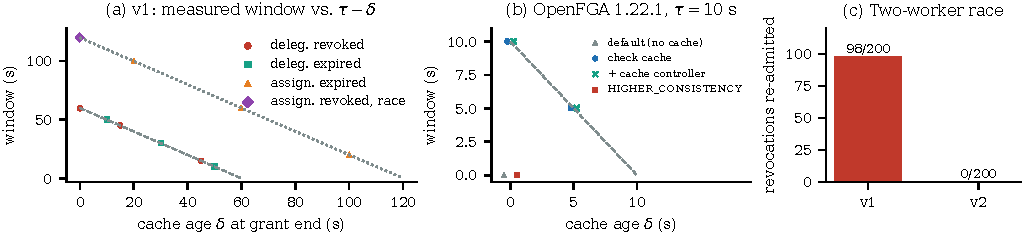
\includegraphics[width=0.92\textwidth]{figs/fig_l2.pdf}
\caption{L2 results. (a) Every v1 staleness trial ($n=10$ per setting) against the prediction $\tau_g-\delta$ of
Theorem~\ref{thm:stale} (dashed: $\tau=60$\,s; dotted: $\tau=120$\,s); the race points use one injected concurrent
decision. (b) OpenFGA, every trial ($n=10$ per setting): with the check cache, with the cache controller added,
with \texttt{HIGHER\_CONSISTENCY}, and in the default configuration; points are offset horizontally for
legibility. (c) Revocations followed by an allow from a re-cached grant under a two-worker server (200 trials
per version).}
\label{fig:l2}
\end{figure*}

\paragraph{Measurements.} Figure~\ref{fig:l2}a and Table~\ref{tab:e2} show ten trials per setting.
Revoking a \emph{delegation} never touches the cache: the windows were 60.1, 45.2, 30.2 and 14.8\,s at
$\delta=0,15,30,45$\,s. Revoking an \emph{assignment} does invalidate, and closed within 0.22\,s with no allowed
decision. \emph{Expiry} is never checked against cached entries, so delegations stayed usable 50.3, 30.2 and
10.3\,s after $t_e$, and assignments 100.3, 60.2 and 20.2\,s after $t_u$. Across all 100 trials, the windows
differ from $\tau_g-\delta$ by between $-0.43$ and $+0.63$\,s, which is about what the 0.25\,s polling interval
and up to 60 concurrent trials should produce (the $\epsilon$ of Theorem~\ref{thm:stale}).

\paragraph{The race.} Assignment revocation invalidates the cache \emph{before} the request transaction commits.
With one decision injected in between, a revoked assignment stayed usable for 120.1 to 120.3\,s ($n=10$).
Without injection, eight decisions racing each revocation in one process left a stale entry in 2 of 60 trials.
We had expected the race to be rare in practice. It is not. Under a server with two workers, \textbf{98 of 200}
revocations (49\,\%; 95\,\% Wilson interval 42--56\,\%) were followed, \emph{after} the revoking request had returned, by an allow decision from a
re-cached grant (Figure~\ref{fig:l2}c). The same harness, run with a single worker during the cost study
(\S\ref{sec:rq5}), counted 174 of 400 (43.5\,\%) in one campaign and 315 of 600 (52.5\,\%) in another: the race
needs concurrent requests, not a second process.
This is adversary class A3: an insider who keeps requesting while an
administrator revokes wins about half the time. Removing a document collaborator behaves like delegation
revocation: no invalidation at all. An open collaboration session is not even consulted. We ran the real
collaboration server against v1, opened a session for a collaborator on a draft, and removed her through the
document API: the API refused her next read at once, but in 10 of 10 trials her session was still open 30\,s
later, with the write permission it had been given at connect (F8).

\begin{table}[t]
\caption{Staleness in v1 ($n=10$ per row): window after the grant ends (median [min, max]) and the largest number
of decisions allowed inside it. Protocol: one decision fills the cache $\delta$ before the grant ends; the window
runs from the return of the revoking request (for expiry, from the end of validity) to the first response of the
decision API that is not an allow, polled with a 0.25\,s pause between requests; the trials of a setting run
concurrently in one server.}
\label{tab:e2}
\footnotesize
\begin{tabular}{@{}l@{\;}r@{\;\;}r@{\;\;}r@{}}
\toprule
Experiment & $\delta$ (s) & window (s) & allows \\
\midrule
Deleg.\ revoked & 0 / 15 & 60.13 [59.59, 60.22] / 45.23 [44.82, 45.44] & 149 / 106 \\
 & 30 / 45 & 30.16 [29.98, 30.28] / 14.84 [14.57, 15.18] & 66 / 27 \\
Deleg.\ expired & 10 / 30 & 50.34 [50.10, 50.63] / 30.24 [30.15, 30.32] & 135 / 82 \\
 & 50 & 10.27 [10.11, 10.50] & 25 \\
Assign.\ expired & 20 / 60 & 100.31 [100.05, 100.44] / 60.24 [60.06, 60.36] & 274 / 156 \\
 & 100 & 20.23 [20.10, 20.40] & 43 \\
Assign.\ revoked & 0 & 0.22 [0.07, 0.22] ($n=5$) & 0 \\
\quad + injected race & 0 & 120.15 [120.09, 120.25] & 453 \\
\bottomrule
\end{tabular}
\end{table}

\paragraph{Mixed views.} We then ran the run of Proposition~\ref{prop:mixed} on the deployment, through the API:
assignment, warming decision, expiry, delegation request and approval, and a write decision 63\,s after the start.
In 10 of 10 trials v1 allowed the write, by $P_4$, and \texttt{/pep/access?action=write} returned
the file, although every committed state of the run denies the request. This allow is not excused by any
staleness tolerance: G1 holds for every $\Delta^\ast$. v2 denied in all 10 trials (by $P_5$), and its file endpoint refused the client-chosen action.

\paragraph{Sessions.} The collaboration server authorizes a WebSocket session once, when it opens. Revoking a
grant has no effect on an open session, so no bound applies on this path at all. Usage control
\cite{park2004ucon} would call this the absence of ongoing authorization.

\answer{2}{With a cold cache, decisions match the stored state. The grant cache keeps revoked or expired grants
usable for $\tau_g-\delta$, as Theorem~\ref{thm:stale} predicts, within 0.63\,s over 100 trials. Invalidating
before the commit lets a race re-admit revoked grants, in 98 of 200 revocations with two workers and in 174 of
400 and 315 of 600 with one; open
collaboration sessions are never re-checked; and because the two grant caches age independently, v1 allowed, in
10 of 10 trials, a write that no committed state allows.}

\subsection{RQ3: The Enforcement Level}
\label{sec:l3}

Reading the code, we found four procedures that decide reads: the \chain PDP, the document service's own
rules, the collaboration server's connect-time check, and a copy of the rules that only decides whether to show
a ``request access'' button; the generated inventory later showed a fifth (F16). Only the decision API and the
file endpoints call the PDP. Table~\ref{tab:l3}
shows the probes that found the failures, and Figure~\ref{fig:l3} the full probe of 57 checks on both versions.

\begin{table*}[t]
\caption{Enforcement probes on the running system, v1 and v2. Ledger cells count durable decision rows per 20
requests; other cells are HTTP status codes. Bold marks a departure from the PDP's decision or from the
requirements.}
\label{tab:l3}
\small
\begin{tabularx}{\textwidth}{@{}p{4.2cm}Xp{1.9cm}p{4.3cm}p{2.3cm}@{}}
\toprule
Probe & Fixture & PDP decision & \sysname v1 & \sysname v2 \\
\midrule
Ledger, \texttt{/pep/access}, \texttt{/preview}, \texttt{/download} & director (allow) / unassigned employee (deny) & allow / deny & allow 20/20; \textbf{deny 0/20 rows}, 0 audit rows & 20/20 and 20/20 \\
Document API \texttt{GET /documents/\{id\}} & published TOP\_SECRET document; employee, \emph{normal} clearance & deny ($\Pc$) & \textbf{200 with full content} (file endpoint on the linked object: 403) & 403 \\
MFA obligation & TOP\_SECRET object; director without MFA & allow ($P_2$) & \texttt{/access} 403; \textbf{\texttt{preview} 200, \texttt{download} 200} & 403 / 403 / 403 \\
Owner bypass & object of another department owned by the requester & deny ($P_1$) & \textbf{\texttt{/access?action=delete} 200; \texttt{download} 200} & 400 / 403 \\
Owner under high risk & own object; $\rho\ge\theta$ (five failed logins, $\theta$ set to 40 for this check) & deny ($\Px$ in $\mathcal{F}$) & \textbf{200} (file and document) & 403 / 403 \\
Change of address & own object and own published document; two failed logins and a new address ($\rho=40$, $\theta$ set to 40) & deny ($\Px$ in $\mathcal{F}$) & \textbf{200} (file and document) & 403 / 403 \\
Deleted object & published document whose object the director deleted; unassigned employee & deny ($P_5$) & \textbf{200 with full content} & 403 \\
Action chosen by the client & assignment \{read\}; \texttt{/pep/download} & deny (download) & \textbf{200 without action parameter} & 403 \\
Revocation authority & unrelated employee of another department & -- & \textbf{revokes a delegation (200) and an assignment (204)} & 403 / 403 \\
Cross-department write & assignment \{read, write\} + read delegation & allow ($P_4$) & \textbf{allowed} (Prop.~\ref{prop:unlock}) & deny \\
Document list \texttt{GET /documents} & published TOP\_SECRET document; employee of the department, \emph{normal} clearance & deny ($\Pc$) & \textbf{listed with full content} & not listed \\
Publishing across departments & approved document; director of another department & deny ($P_1$) & \textbf{200, document published} & 403 \\
\bottomrule
\end{tabularx}
\end{table*}

\begin{figure*}[t]
\centering
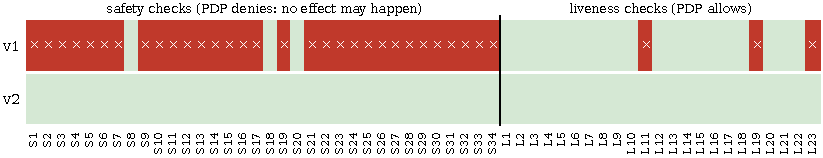
\includegraphics[width=0.92\textwidth]{figs/fig_l3.pdf}
\caption{The L3 probe on v1 and v2: 34 safety checks (S) and 23 liveness checks (L), one run each; a cross marks a
failed check. v1 fails 31 safety checks and three liveness checks. L19 fails because comment resolution always
failed with a server error in v1, L23 only because S33 had already published the document, and L11 only because an unauthorised
director had already revoked the delegation in S15. S19 and S21 use states created through the ORM (a division
manager without a division; a statement-level grant update) that the API of v1 does not produce.}
\label{fig:l3}
\end{figure*}

\paragraph{Lost denials.} The file endpoints write the decision, raise HTTP 403, and let the request
transaction roll back. Every denial disappears together with its audit entry, while the error message tells
the user that the denial ``is permanently logged''. This one embarrassed us most, because denials are precisely
what an investigator needs, and it is what adversary class A6 relies on. The ledger is not append-only either:
deleting a subject cascades into it, and the retention job crashes at run time on a column that does not
exist. Webhook notifications of denials fail too, because they reuse the request's session after it has been
committed.

\paragraph{Paths around the PDP.} The document API lets any employee read any published document of their
department, without an assignment and without the classification test, so it violates R2 and R3, which the PDP
provably satisfies. Unpublished documents fare no better: a collaborator with \emph{normal} clearance reads a
TOP\_SECRET draft, and a division manager reads a TOP\_SECRET department-level document under review. The
collaboration server lets anyone in the department read any document. The owner bypass grants every action
before the PDP runs, attaches no obligations and ignores risk; and since ownership survives a move to another
department, it breaks R1 for owners. Obligations are enforced on one of the three file endpoints, and the
download endpoint evaluates whichever action the client sends.

\paragraph{Administration.} The PDP never reads a policy's status, so the PAP can show a rule as inactive while
it is enforced. The PAP's guard against disabling $P_7$ exists on one of its two update routes, and any
authenticated user can revoke anyone's grants.

\paragraph{Routes we had not listed.} All of the above came from an inventory we had built by reading the code.
We then generated it from the web framework's routing table: 152 API routes, plus four documentation routes and a
metrics endpoint. A static pass over the handlers marks a route as in scope if it can touch an object, a document
or a part of one, return content, or change a grant; 100 are. For each it records which decision procedures the
handler can reach; for v1, six in-scope routes reach none. Four of those are known or deliberate (the revocation
of F14; an access graph documented as visible to everyone; aggregate statistics; document templates); the other
two, comment resolution and signing, are new. Because reaching a procedure does not
mean applying it to the right object, we added two sweeps that need no per-route fixtures. The first sends every
in-scope GET route (48) as an employee of another department and as an unassigned employee of the owning
division, with every text field of the objects marked by kind; the second sends every state-changing route (52)
as those two and as a director and a division manager of another department, against documents in every workflow
state, and compares the database before and after. Together they found four failures (F15--F18 in
Table~\ref{tab:findings}): comment resolution and signing decide nothing; the document list is a fifth decision
procedure, a database query that returns every published document of the department with its content and
ignores $\Pc$, so a TOP\_SECRET document reaches an employee with \emph{normal} clearance; any subject reads any
delegation; and directors and division managers publish, escalate and remove another department's documents and
folders. On v1 the state sweep flags ten routes; on v2 it flags one, because an employee may create a folder in
her own department's space, which no requirement covers. The sweeps also show names and titles of objects the
subject may not read, on six routes of v1 and five of v2. R constrains actions on objects, not their names, so we report these and do not count them as
violations. Nine creation
routes rejected the sweep's minimal bodies (HTTP 422) and one takes a file upload; these ten were not exercised.

\paragraph{Summary of findings.} Table~\ref{tab:findings} collects the eighteen findings of
\S\ref{sec:l1}--\S\ref{sec:l3} and the adversary class each one serves. Fourteen of them lie outside the decision
function.

\begin{table}[t]
\caption{Findings on \sysname v1, by level, adversary class (Table~\ref{tab:adv}) and evidence (P proof; X
exhaustive count; R reproduced on the running system; C code inspection). All are fixed in v2
(\S\ref{sec:rq5}). F15--F18 were found only after the route inventory was generated.}
\label{tab:findings}
\small
\begin{tabularx}{\columnwidth}{@{}l@{\;}l@{\;}l@{\;}X@{\;}l@{}}
\toprule
ID & Lvl & Cl. & Finding & Ev. \\
\midrule
F1 & L1 & A1 & Risk rule $\Px$ never decides (Prop.~\ref{prop:inert}) & P,X \\
F2 & L1 & A1 & $P_5$ shadows employee delegations (R4) & P,X \\
F3 & L1 & A1 & Read delegation unlocks cross-department writes & P,X,R \\
F4 & L1 & A1 & Spec drift D1--D3; least-privilege theorem false & P,X \\
F5 & L2 & A2 & Delegation revocation and collaborator removal never invalidate & R,C \\
F6 & L2 & A2 & Validity bounds ignored for cached grants & R \\
F7 & L2 & A3 & Invalidation before commit re-admits revoked grants (44--53\,\% of trials) & R \\
F8 & L2 & A2 & Collaboration sessions authorized only at connect & R,C \\
F9 & L2 & A2 & Mixed cached views allow what no committed state allows & P,R \\
F10 & L3 & A6 & Denials rolled back; ledger not append-only; retention job crashes & R,C \\
F11 & L3 & A4 & Document API and collaboration server bypass the PDP & R,C \\
F12 & L3 & A5 & Owner bypass grants every action, ignores risk, survives a change of department & R \\
F13 & L3 & A4 & Obligations on one endpoint only; client chooses the action & R \\
F14 & L3 & A7 & PAP status ignored by the PDP; revocation needs no authority & R,C \\
F15 & L3 & A4 & Comment resolution and signing call no decision procedure & R,C \\
F16 & L3 & A4 & Document list decides on its own: content of every published document, no $\Pc$ & R \\
F17 & L3 & A4 & Any subject reads any delegation & R \\
F18 & L3 & A4 & Publishing, escalation and folder removal across departments & R \\
\bottomrule
\end{tabularx}
\end{table}

\answer{3}{Five procedures decide reads, and only the decision API and the file endpoints ask the PDP. The
document API, the document list and the collaboration server bypass it, the owner rule skips it, obligations
are enforced on one of three file endpoints, the client chooses the action, denials are never recorded, anyone
can revoke grants, and several routes decide nothing or ignore the department. Fourteen of the eighteen findings
lie outside the decision function, and four of them appeared only once the route inventory was generated from
the routing table instead of read from the code.}

